\documentclass[12pt]{article}
\usepackage{amsmath, amssymb, amsthm, commath, enumitem, graphicx, nopageno, quoting}
\usepackage[margin=1cm]{geometry}

\graphicspath{ {./images/} }

\title{Computer Science 452 - Homework Assignment \#2}
\author{Hari Amoor, NetID: hra25}
\date{February 4, 2020}

\begin{document}
\maketitle

\section*{Problem 1.7c: Supply a state diagram for an NFA with six states that recognizes the language of words containing either an even number of 0s or at least two 1s.}
The state diagram is as follows: \\
\newline
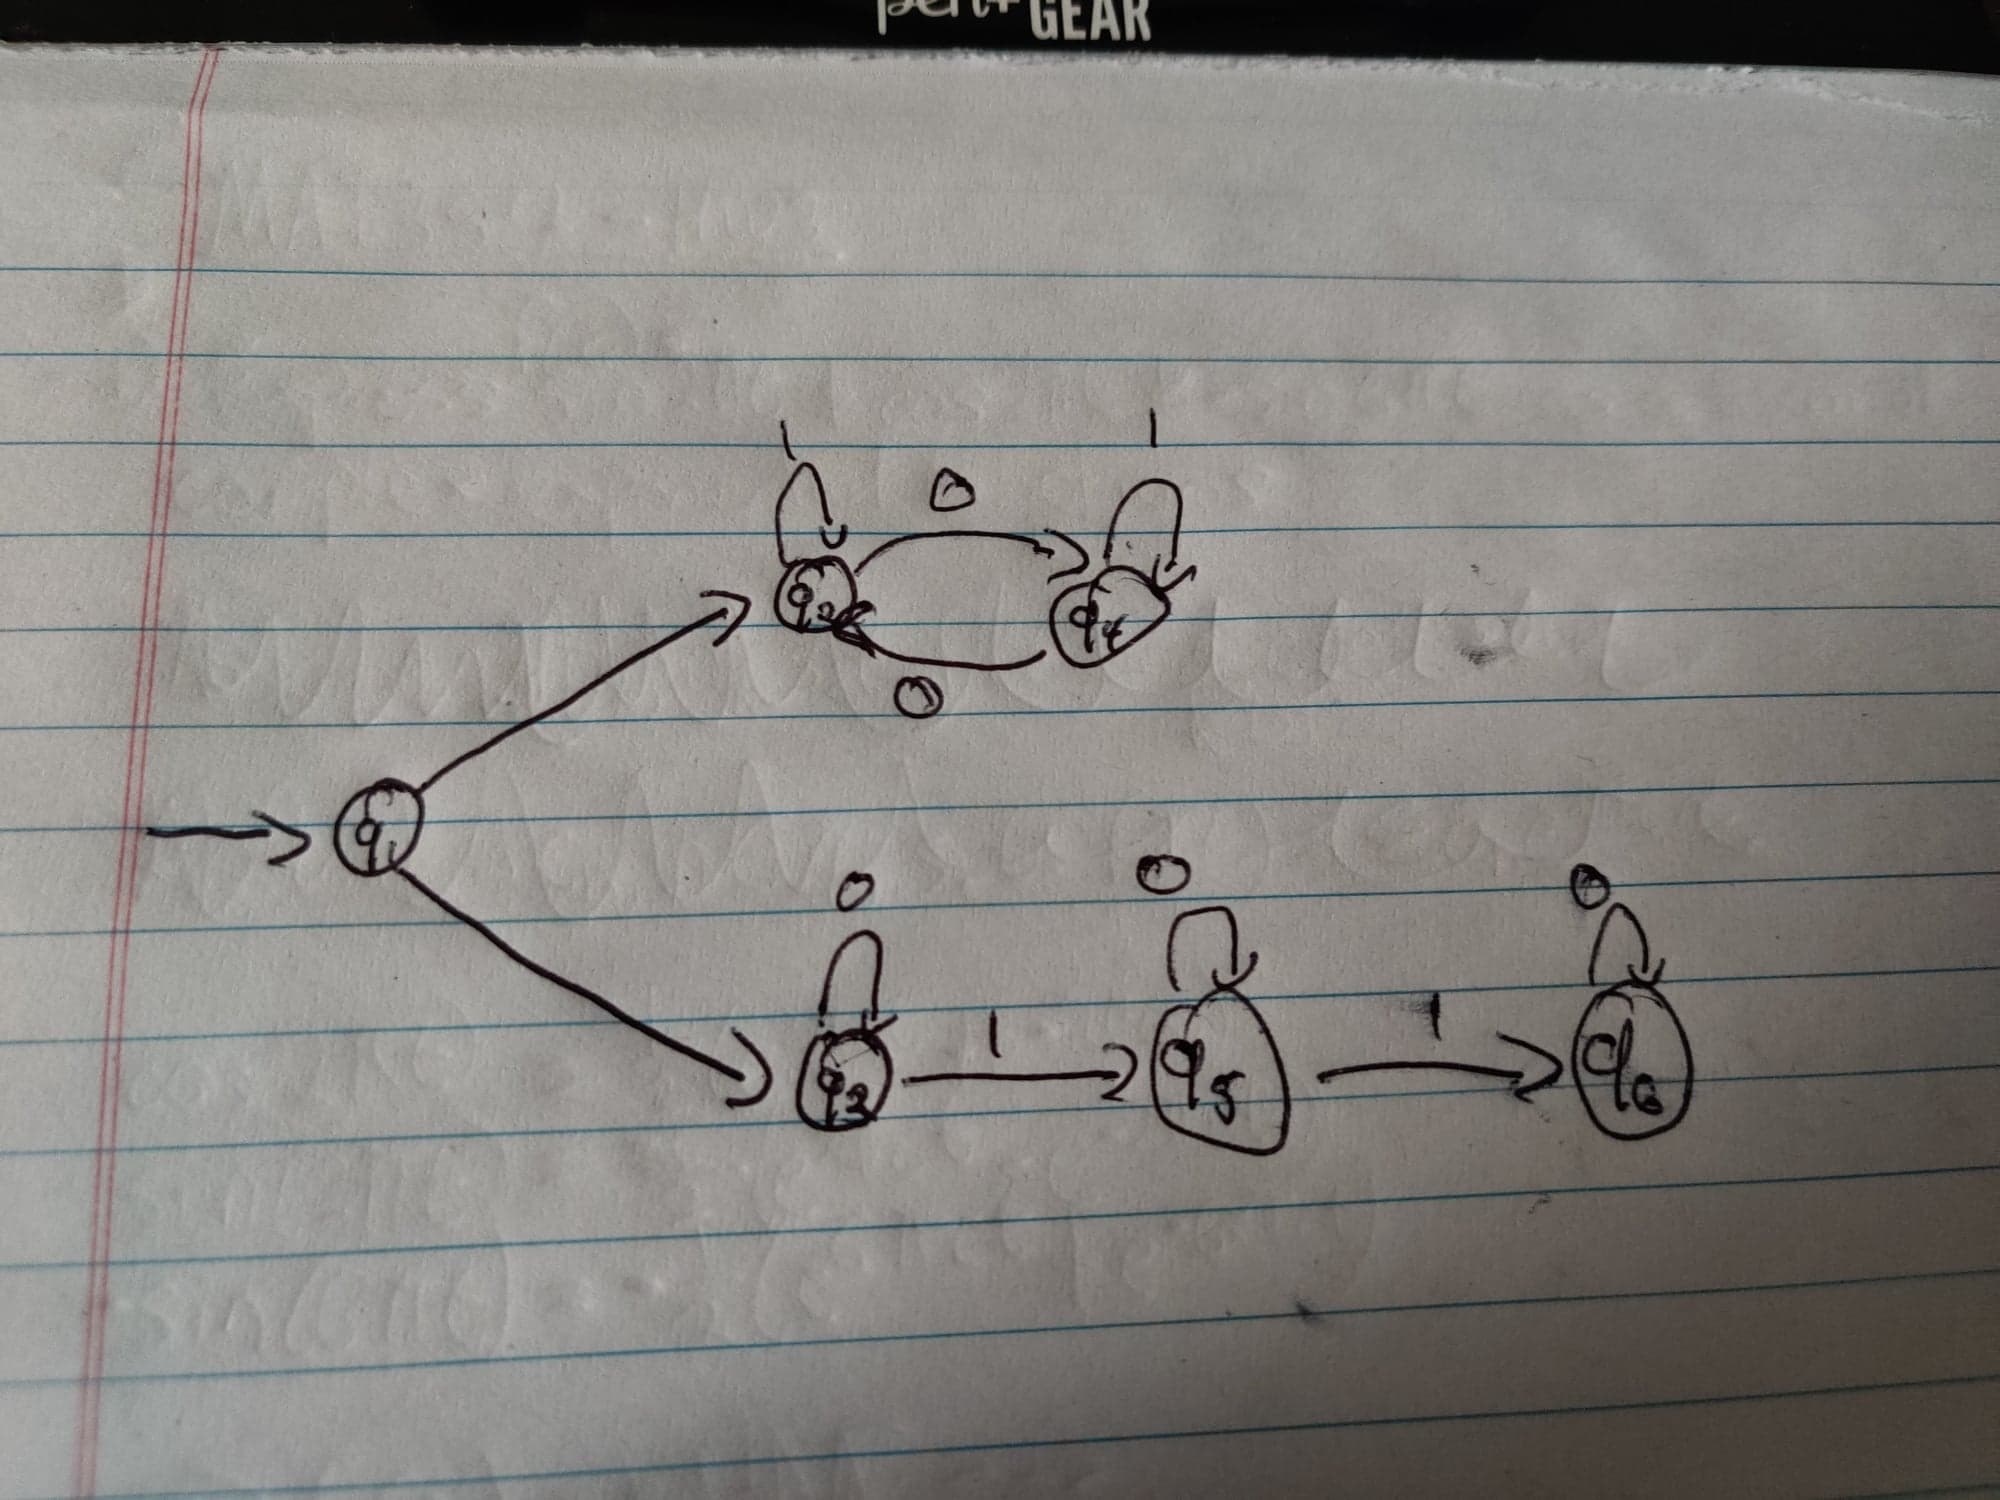
\includegraphics[width=0.5\linewidth]{problem17c.jpg}

\section*{Problem 1.10a: Supply a state diagram for an NFA that recognizes $\{w* \mid w \text{ contains at least three 1s}\}$.}
The state diagram is as follows:
\newline
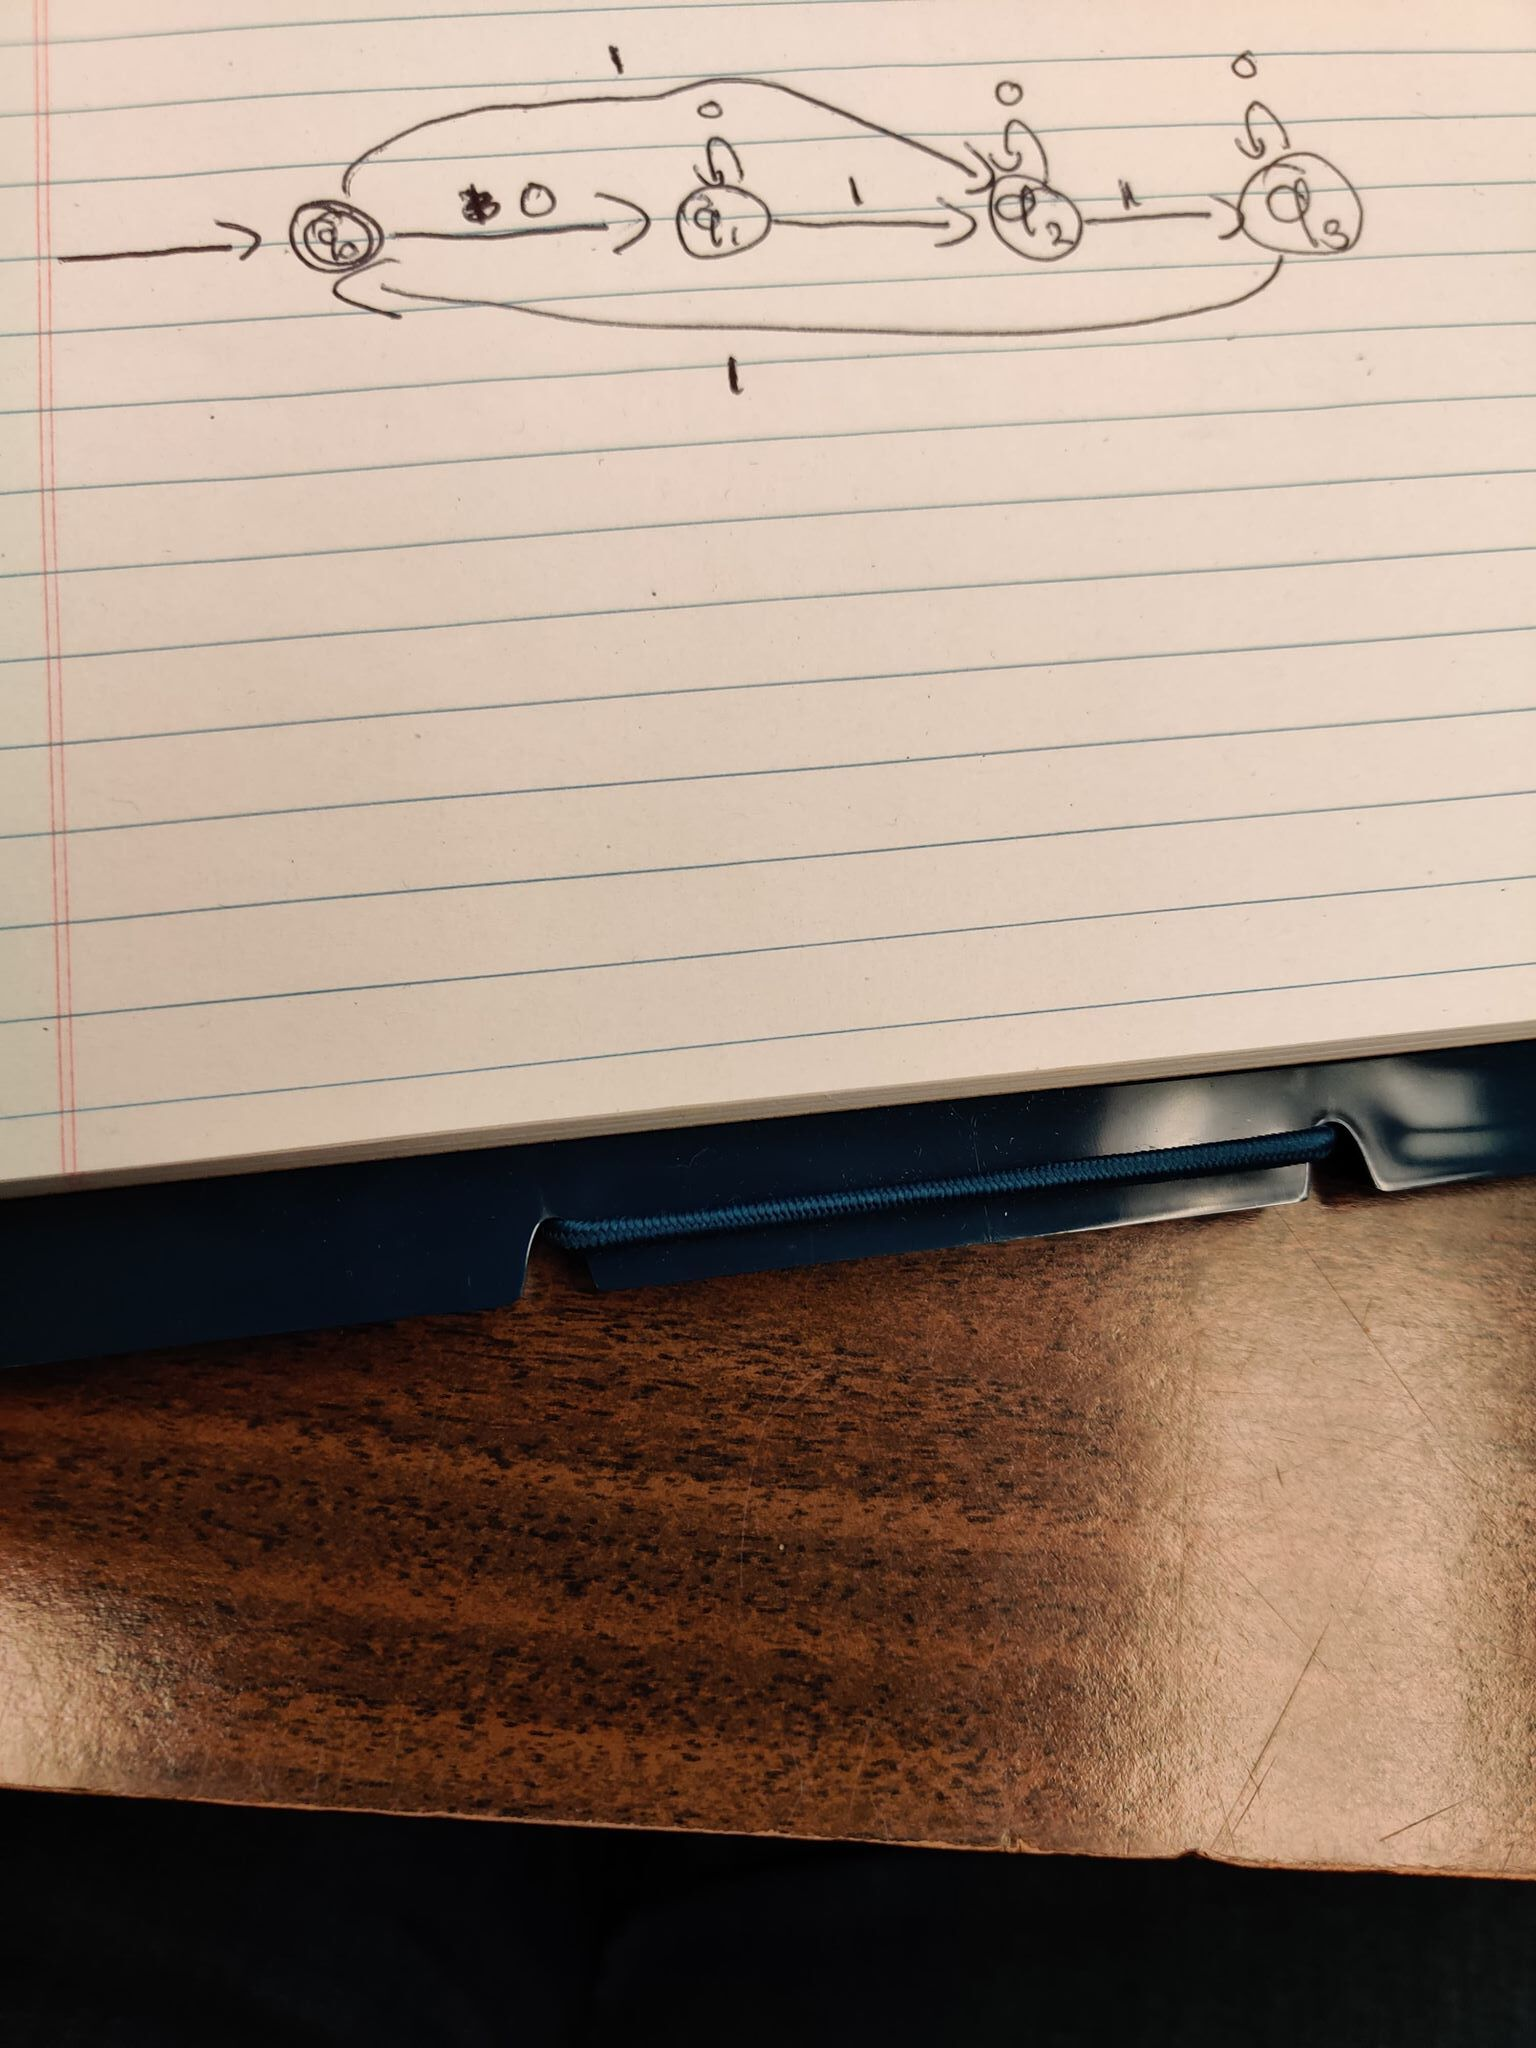
\includegraphics[width=0.5\linewidth]{problem110a.jpg}

\section*{Problem 1.14b: Show that swapping the accept and non-accept states of an NFA that recognizes a language $L$ does not necessarily form an NFA that recognizes $L^{\complement}$. Is the class of languages recognized by NFAs closed under complement?}
Consider the following NFA: \\
\newline
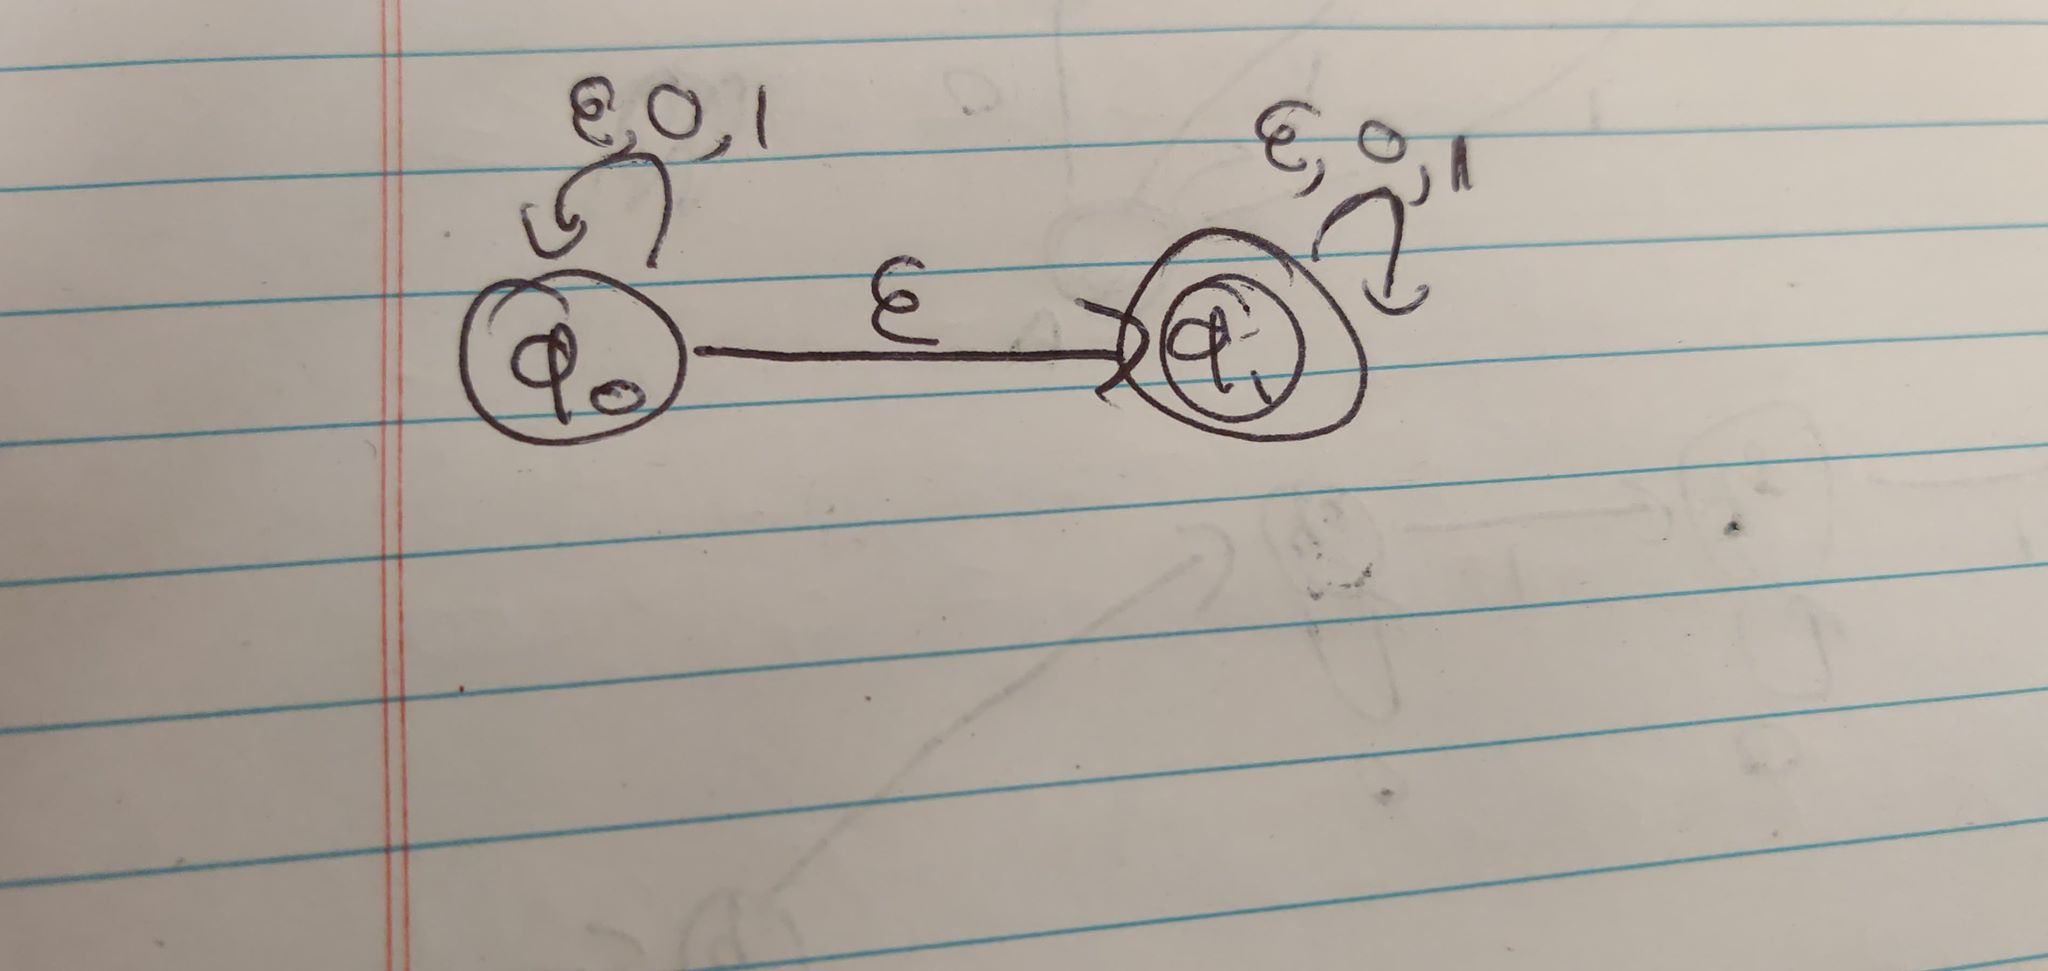
\includegraphics[width=0.5\linewidth]{problem114b.jpg} \\
\newline
The string $\varepsilon$ is recognized in both the given NFA and the NFA obtained with switching the accept and non-accept states of the given, as required. However, the class of languages recognized by NFAs is closed under complement, as demonstrated. \\
\begin{proof}
	Let $M$ be an NFA. We know that an equivalent DFA $M'$ exists, i.e. $L(M) = L(M')$. Trivially, there must exist a DFA $N$ that recognizes the complement of $L(M')$. $N$ is an NFA that recognizes the complement of $L(M') = L(M)$, as required.
\end{proof}

\section*{Problem 1.15: Show that the given construction does not prove that the set of languages recognized by an NFA is closed under the Kleene star.}
Consider the following NFA: \\
\newline
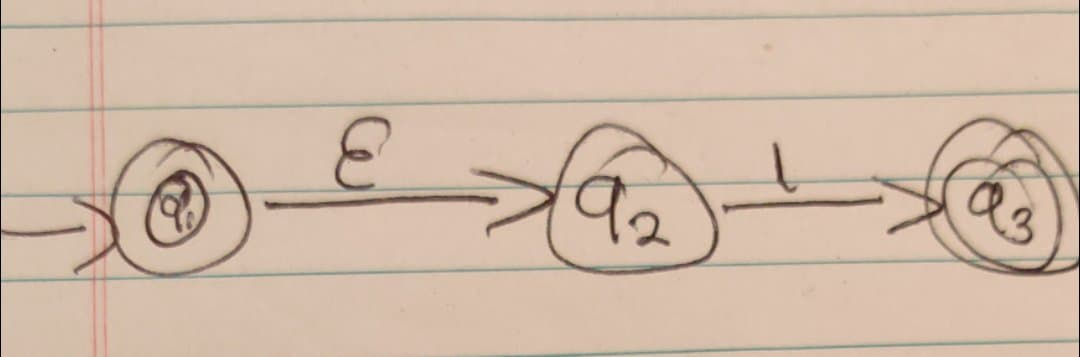
\includegraphics[width=0.5\linewidth]{problem115i.jpg} \\
\newline
The NFA constructed with the given rules , is as follows: \\
\newline
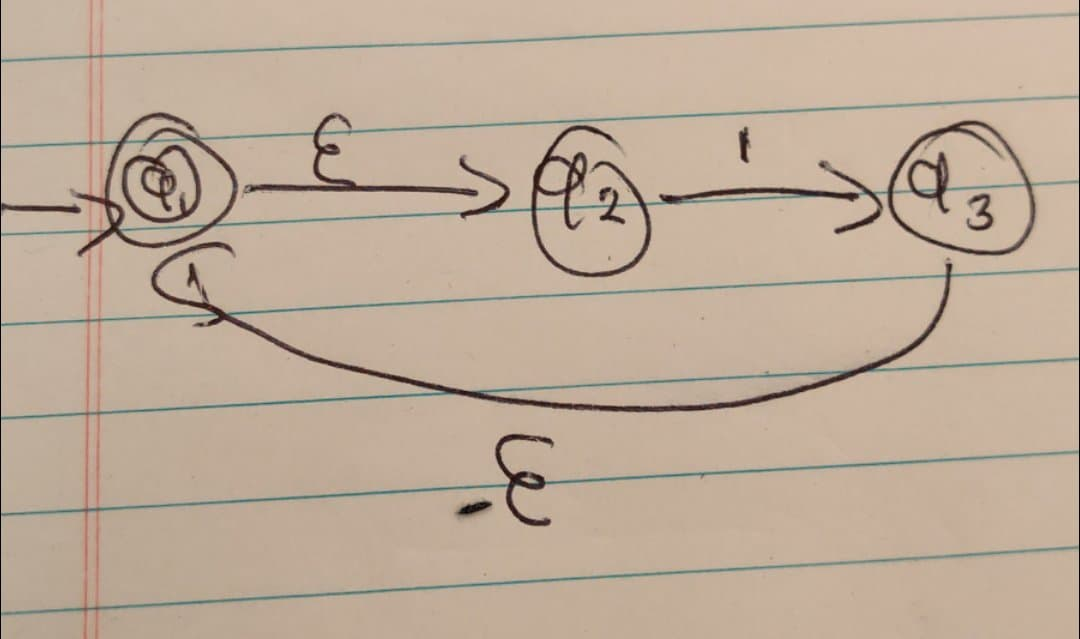
\includegraphics[width=0.5\linewidth]{problem115ii.jpg} \\
\newline
Clearly, it fails at $\varepsilon$, and thus does not recognize the Kleene-closure of the language of the initial NFA.

\section*{Problem 1.16b: Supply a DFA equivalent to the given NFA.}
This is given below: \\
\newline
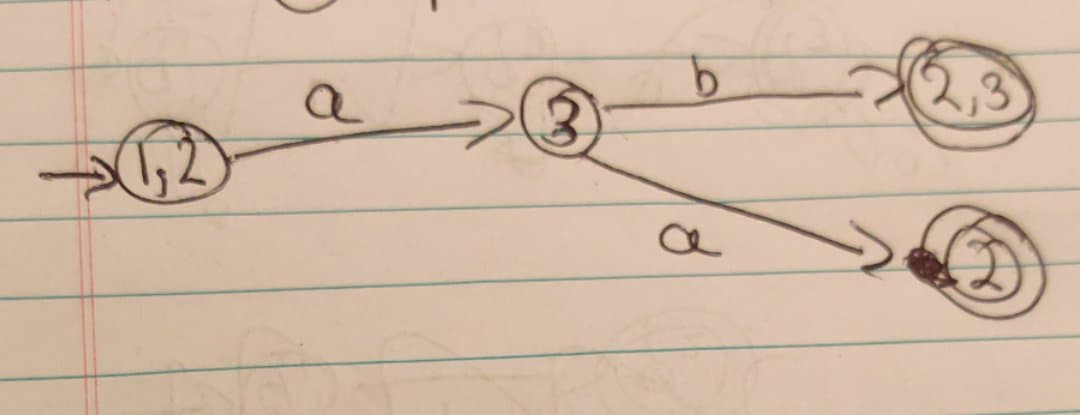
\includegraphics[width=0.5\linewidth]{problem116b.jpg}

\section*{Problem 1.17: Complete the following.}
\begin{enumerate}[label=(\alph*)]
	\item \textbf{Supply an NFA for the given language.} \\
		\newline
		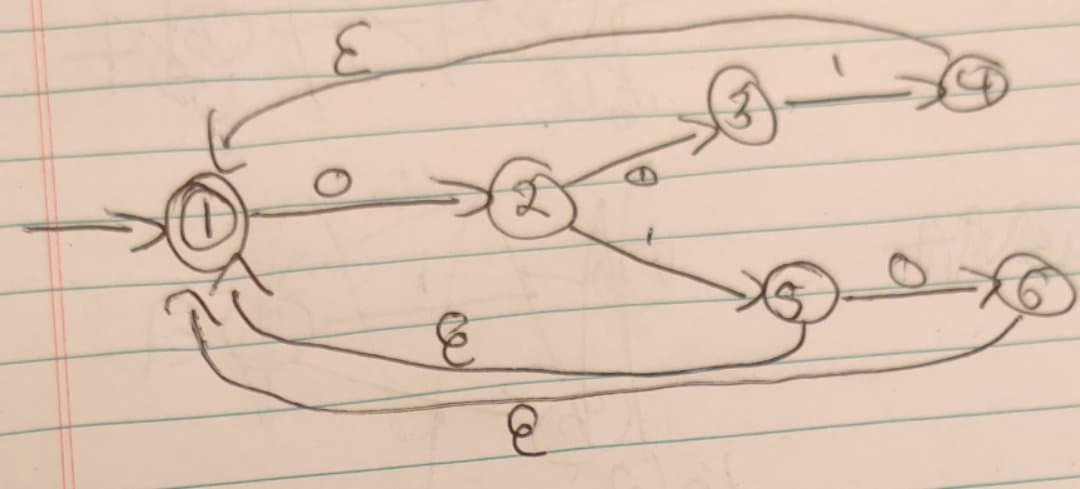
\includegraphics[width=0.5\linewidth]{problem117a.jpg}
	\item \textbf{Convert the NFA from (a) to a DFA.} \\
		\newline
		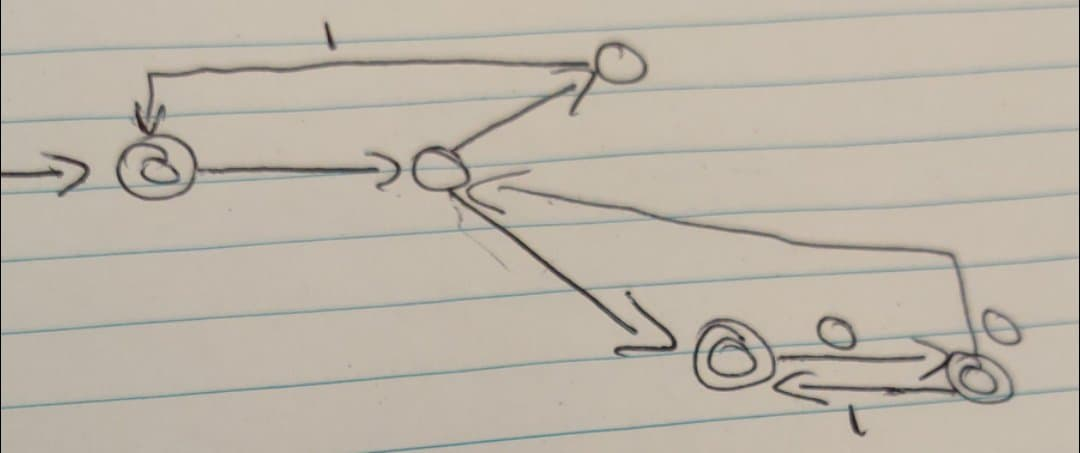
\includegraphics[width=0.5\linewidth]{problem117b.jpg}
\end{enumerate}

\section*{Problem 1.18: For parts (i) and (l), supply regular expressions detecting the given language.}
For Part (i), the regular expression $(10 \cup 11)^{*}$ describes the language. For Part (l), the regular expression $((ab^{*}ab^{*})^{*} \cup 01^{*}01^{*})$ describes the given language.

\section*{Problem 1.31, Claim: If $A$ is regular, then so is $A^{R}$.}
\begin{proof}
	Let $A$ be a regular language, and suppose the DFA $M$ has $L(M) = A$. Suppose w.l.o.g. that $M = (Q, \Sigma, \delta, q_{0}, \{f\})$, i.e. $M$ only has one accepting state. Then, the DFA $M' = (Q, \Sigma, \delta^{R}, \{f\}, \{q_{0}\})$ recognizes $A^{R}$. Here, $\delta^{R}$ is the transition relation defined by $\delta(q, a) \mapsto q$, i.e. the $\it{reversed}$ transitions of $\delta$. \\
	\newline
	$M'$ as defined recognizes $A^{R}$, as required.
\end{proof}

\section*{Problem 1.34: Show that the given language is regular.}
The given language is recognized by the following DFA: \\
\newline
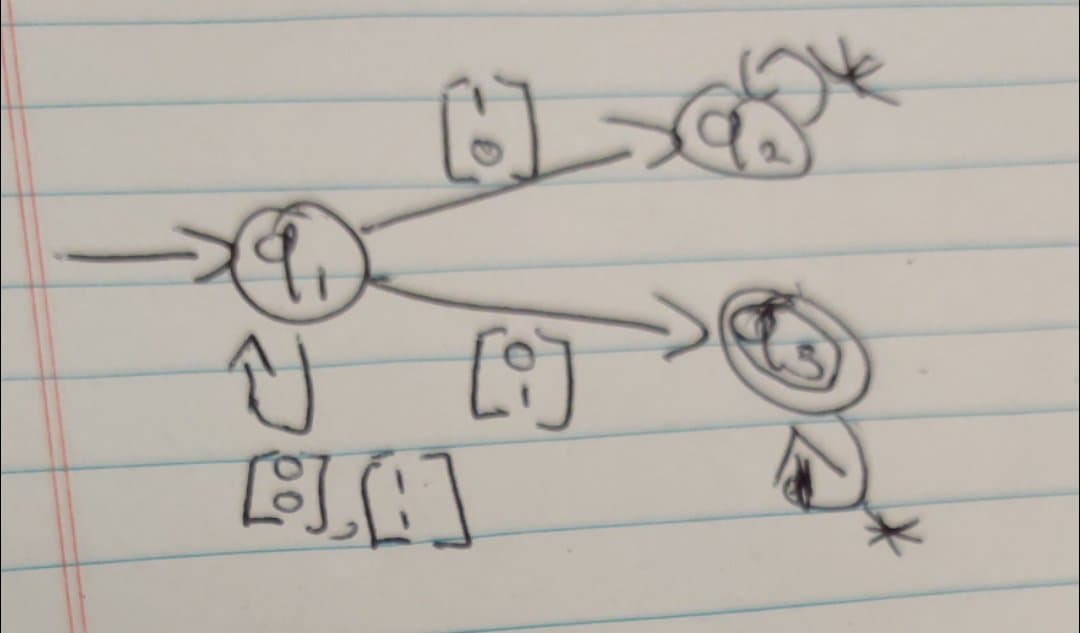
\includegraphics[width=0.5\linewidth]{problem134.jpg}

\section*{Problem 1.51, Claim: $\equiv_{L}$ is an equivalence relation.}
\begin{proof}
	We show that $\equiv_{L}$ is reflexive, symmetric and transitive. \\
	\newline
	Let $x$ be a string and $w \in L$ be arbitrary for some language $L$. In general, either $xw \in L$ or $xw \notin L$. So, $x \equiv_{L} x$ for all strings $x$. Therefore, $\equiv_{L}$ is reflexive. \\
	\newline
	Let $x, y$ be strings. Suppose that $x \equiv_{L} y$; then, for all $w \in L$, either $xw, yw \in L$ or $xw, yw \notin L$. Equivalently, $yw, xw \in L$ or $yw, xw \notin L$. Thus, $y \equiv_{L} x$, so $\equiv_{L}$ is symmetric. \\
	\newline
	Let $x, y, z$ be strings, and suppose $x \equiv_{L} y$ and $y \equiv_{L} z$. Then, for all $w \in L$, $xw \in L$ iff $yw \in L$, and $yw \in L$ iff $zw \in L$. Thus, $xw \in L$ iff $zw \in L$ for all $w$. Thus, $\equiv_{L}$ is transitive, as required.
\end{proof}


\end{document}
